\section{Introduction}

The final state consisting of a low transverse energy photon and low missing transverse energy (\met) (also called the ``monophoton'' final state) can be used to constrain a variety of extensions of the standard model (SM). One such promising extension is supersymmetry (SUSY)~\cite{GGMa,GGMd2,GGMd3,GGMd4,GGMd5,GGMd1,GGMd}, which has the attractive feature of stabilizing the radiative corrections to the Higgs boson mass ($m_{h}$), while also providing a natural dark matter (DM) particle candidate ($\chi$) in the form of the lightest supersymmetric particle (LSP). 

\begin{figure}[h]
\centering
{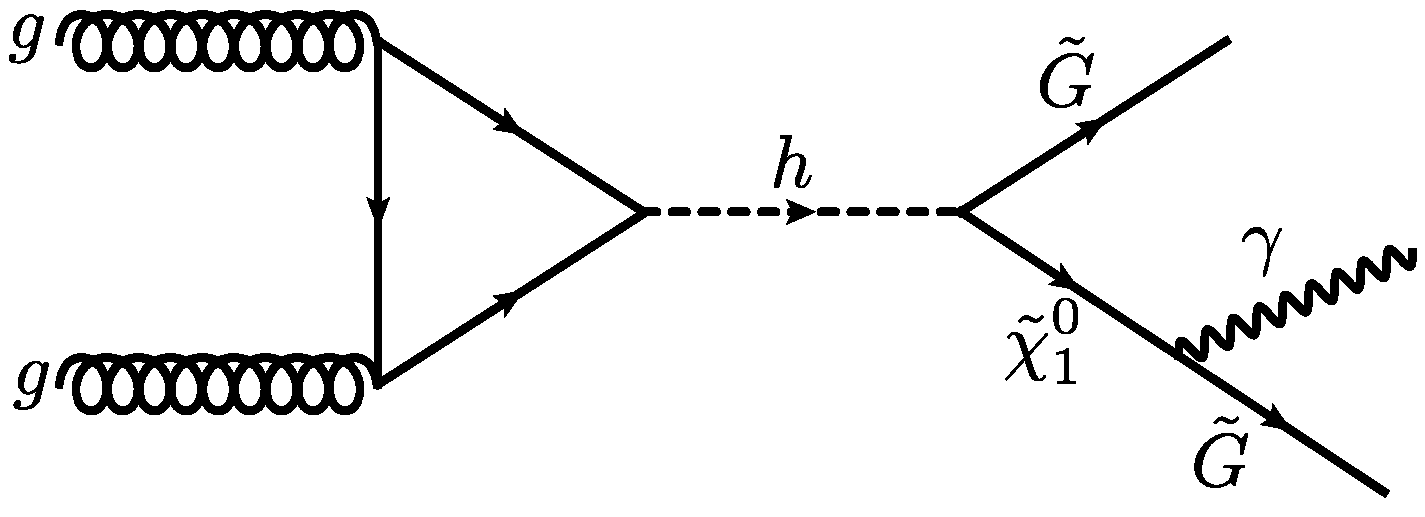
\includegraphics[width=0.55\columnwidth]{figures/susy_feynman}}
\caption{Feynman diagrams of a Higgs boson decay to gravitino LSP and a neutralino NLSP, which subsequently decays to a gravitino and photon.
}
\label{fig:feynman}
\end{figure}

In SUSY scenarios where the SUSY breaking scale is low ($\sqrt{f} \sim \TeV$ ) the newly discovered Higgs boson ($m_h = 125 \GeV$) \cite{cmshiggs,atlashiggs} may decay into a gravitino (\PXXSG) and neutralino (\PSGczDo), with the neutralino subsequently decaying into a gravitino and a photon~\cite{Petersson:2012dp}. In this model, the gravitino is the LSP and the neutralino is the next-to-lightest supersymmetric particle (NLSP). Figure~\ref{fig:feynman} shows the Feynman diagram for this process. 

The fact that the gravitino is massive and stable (as the LSP) can give rise to cosmological problems (often quoted as the gravitino problem). 
This problem is related to the fact that the energy density of the gravitinos, which are produced in the early universe, may exceed the present critical density of the early universe if the gravitino mass is larger than 1 keV \cite{grav_prob}. 
The benchmark model for this analysis, however, circumvents this issue with the fact that $\sqrt{f} \sim \TeV$. 
This gives a gravitino mass that is $m_{3/2} \approx f/\sqrt{3}M_{P} \approx 10^{-3}$ eV, much smaller than the critical gravitino mass.

%In order for the gravitino-neutralino-higgs coupling vertex to be allowed, the gravitino must be approximately massless ($m_{\PXXSG} \sim f / M_{P} \sim 10^{-3}$ eV) so that by the supersymmetric equivalence theorem the gravitino (spin $3/2$) can be represented by its goldstino (spin $1/2$) component \cite{higgs-gravitino-neutralino}. 

This decay mode produces a single isolated photon and \met from the undetected gravitinos. If $m_{\PSGczDo} < m_{h}/2$, the decay process $h \to \PSGczDo \PSGczDo \to \gamma \gamma + \met$ would dominate. Therefore the kinematic region of interest for this search is $m_{h}/2 < m_{\PSGczDo} < m_{h}$. Furthermore, since $m_{h} = 125 \GeV$, the photon transverse energy (\etg) and \met will be relatively low. 

In this document, we present a search for new physics in the low-\et photon+\met final state, using an integrated luminosity at 7.3\fbinv of $\sqrt{s}=8\TeV$ LHC pp collision data collected with the CMS detector. This study is the first CMS search conducted in this low energy regime and it complements and expands upon previous high-energy monophoton searches for new physics conducted at the LHC~\cite{Chatrchyan:2012tea,Aad:2012fw}. The results are interpreted in terms of the low-scale SUSY breaking model, as well as in a model independent manner.

  %%---- DM
%  Final states involving  a $\gamma$ and \ETslash has been studied previously for various signature proposed for new physics beyond SM~\cite{Chatrchyan:2012tea,Aad:2012fw}. 
%The $\gamma$+\met final state has also been used to search for DM, in particular a DM candidate for the dominant non-baryonic contribution to the matter density of the universe ~\cite{DMGeneral, Chatrchyan:2012tea,Aad:2012fw}.
%One of the most sought scenario is  model for dark matter (DM), which could be a candidate for the dominant non-baryonic contribution to the matter density of the universe~\cite{DMGeneral}. 
%Many experiments have searched for signatures of DM candidates ($\chi$) using elastic $\chi$-nucleon scattering~\cite{CDMS2,XENON100,PICASSO,COUPP,COGENT,CDMSLITE,LUX}. Indirect searches consist of observation of photons or neutrinos produced in $\chi\overline{\chi}$ annihilations in astrophysical sources[FIXME].

%At hadron colliders such as the LHC, DM particles could be produced in the process $\Pq\Paq \rightarrow  \Pgg \chi\overline{\chi}$, where the photon is radiated by one of the incoming initial state quarks (Fig~\ref{fig:feynDM}). This process can be expressed in a theoretical framework in which a massive ``mediator'' particle in the $s$-channel couples to a pair of $\chi$ particles. An effective field theory (EFT) approach could be used to describe this process with an energy or interaction scale $\Lambda$~\cite{DMGeneral,DMTeva, Majorana_dm,DMCollid}. The mass of the mediator particle $M$, its coupling ($g_{\chi}$) to quarks and to DM pairs ($g_\Pq$) could be expressed as: $\Lambda^{-2} = g_{\chi}g_qM^{-2}$. The EFT approach provides a way to compare the  $t$-channel $\chi$-nucleon elastic scattering to the $s$-channel pair-production mechanism. The effective $s$-channel operator can be chosen to represent either vector or axial-vector, i.e., spin-independent or spin-dependent, interactions respectively. These operators are some of the lowest dimensional operators and for simplicity are used here as done previously in the literature [FIXME]. The $\chi$-nucleon cross section can be express in terms of $M_{\chi}$, $\Lambda$, and reduced mass $\mu$ with the following relations:

%\begin{equation}
%\label{eq:dmXS}   
%\sigma_{SI} = 9\frac{\mu^{2}}{\pi\Lambda^{4}} ,       
%\sigma_{SD} = 0.33 \frac{\mu^{2}}{\pi\Lambda^{4}} 
%\end{equation}

